\documentclass[12pt]{article}\usepackage[]{graphicx}\usepackage[]{color}
%% maxwidth is the original width if it is less than linewidth
%% otherwise use linewidth (to make sure the graphics do not exceed the margin)
\makeatletter
\def\maxwidth{ %
  \ifdim\Gin@nat@width>\linewidth
    \linewidth
  \else
    \Gin@nat@width
  \fi
}
\makeatother

\definecolor{fgcolor}{rgb}{0.345, 0.345, 0.345}
\newcommand{\hlnum}[1]{\textcolor[rgb]{0.686,0.059,0.569}{#1}}%
\newcommand{\hlstr}[1]{\textcolor[rgb]{0.192,0.494,0.8}{#1}}%
\newcommand{\hlcom}[1]{\textcolor[rgb]{0.678,0.584,0.686}{\textit{#1}}}%
\newcommand{\hlopt}[1]{\textcolor[rgb]{0,0,0}{#1}}%
\newcommand{\hlstd}[1]{\textcolor[rgb]{0.345,0.345,0.345}{#1}}%
\newcommand{\hlkwa}[1]{\textcolor[rgb]{0.161,0.373,0.58}{\textbf{#1}}}%
\newcommand{\hlkwb}[1]{\textcolor[rgb]{0.69,0.353,0.396}{#1}}%
\newcommand{\hlkwc}[1]{\textcolor[rgb]{0.333,0.667,0.333}{#1}}%
\newcommand{\hlkwd}[1]{\textcolor[rgb]{0.737,0.353,0.396}{\textbf{#1}}}%
\let\hlipl\hlkwb

\usepackage{framed}
\makeatletter
\newenvironment{kframe}{%
 \def\at@end@of@kframe{}%
 \ifinner\ifhmode%
  \def\at@end@of@kframe{\end{minipage}}%
  \begin{minipage}{\columnwidth}%
 \fi\fi%
 \def\FrameCommand##1{\hskip\@totalleftmargin \hskip-\fboxsep
 \colorbox{shadecolor}{##1}\hskip-\fboxsep
     % There is no \\@totalrightmargin, so:
     \hskip-\linewidth \hskip-\@totalleftmargin \hskip\columnwidth}%
 \MakeFramed {\advance\hsize-\width
   \@totalleftmargin\z@ \linewidth\hsize
   \@setminipage}}%
 {\par\unskip\endMakeFramed%
 \at@end@of@kframe}
\makeatother

\definecolor{shadecolor}{rgb}{.97, .97, .97}
\definecolor{messagecolor}{rgb}{0, 0, 0}
\definecolor{warningcolor}{rgb}{1, 0, 1}
\definecolor{errorcolor}{rgb}{1, 0, 0}
\newenvironment{knitrout}{}{} % an empty environment to be redefined in TeX

\usepackage{alltt}
\usepackage{amsmath}
\usepackage{amssymb}
\usepackage{graphicx}
\setlength{\textheight}{10.1in}
\setlength{\topmargin}{-1.2in}
\setlength{\textwidth}{7in}
\setlength{\oddsidemargin}{-0.25in}
\newcommand{\zsp}{\rule{0pt}{5pt}}
\newcommand{\ind}{\zsp\hspace{6mm}}
\newcommand{\bzr}{{\bf 0}}
\newcommand{\ba}{{\bf a}}
\newcommand{\bb}{{\bf b}}
\newcommand{\bc}{{\bf c}}
\newcommand{\be}{{\bf e}}
\newcommand{\bs}{{\bf s}}
\newcommand{\bp}{{\bf p}}
\newcommand{\bx}{{\bf x}}
\newcommand{\by}{{\bf y}}
\newcommand{\bz}{{\bf z}}
\newcommand{\bu}{{\bf u}}
\newcommand{\bv}{{\bf v}}
\newcommand{\bw}{{\bf w}}
\newcommand{\yp}{\frac{dy}{dt}}
\newcommand{\ypp}{\frac{d^2y}{dt^2}}
\newcommand{\Dint}{\displaystyle\int}
\IfFileExists{upquote.sty}{\usepackage{upquote}}{}
\begin{document}
\LARGE
\thispagestyle{empty}

\subsection{Population Growth Models}

\begin{knitrout}
\definecolor{shadecolor}{rgb}{0.969, 0.969, 0.969}\color{fgcolor}\begin{kframe}
\begin{alltt}
\hlstd{day} \hlkwb{=} \hlkwd{c}\hlstd{(}\hlnum{0}\hlstd{,} \hlnum{1}\hlstd{,} \hlnum{2}\hlstd{,} \hlnum{3}\hlstd{,} \hlnum{4}\hlstd{,} \hlnum{5}\hlstd{,} \hlnum{6}\hlstd{,} \hlnum{7}\hlstd{,} \hlnum{8}\hlstd{,} \hlnum{9}\hlstd{,} \hlnum{10}\hlstd{)}
\hlstd{N} \hlkwb{=} \hlkwd{c}\hlstd{(}\hlnum{10}\hlstd{,} \hlnum{14}\hlstd{,} \hlnum{19}\hlstd{,} \hlnum{24}\hlstd{,} \hlnum{28}\hlstd{,} \hlnum{38}\hlstd{,} \hlnum{55}\hlstd{,} \hlnum{72}\hlstd{,} \hlnum{85}\hlstd{,} \hlnum{123}\hlstd{,} \hlnum{136}\hlstd{)}
\hlstd{q1.df} \hlkwb{=} \hlkwd{data.frame}\hlstd{(}\hlkwc{Day} \hlstd{= day,} \hlkwc{Population} \hlstd{= N)}
\end{alltt}
\end{kframe}
\end{knitrout}

\begin{knitrout}
\definecolor{shadecolor}{rgb}{0.969, 0.969, 0.969}\color{fgcolor}\begin{kframe}
\begin{alltt}
\hlkwd{plot}\hlstd{(Population} \hlopt{~} \hlstd{Day,} \hlkwc{data}\hlstd{=q1.df)}
\end{alltt}
\end{kframe}
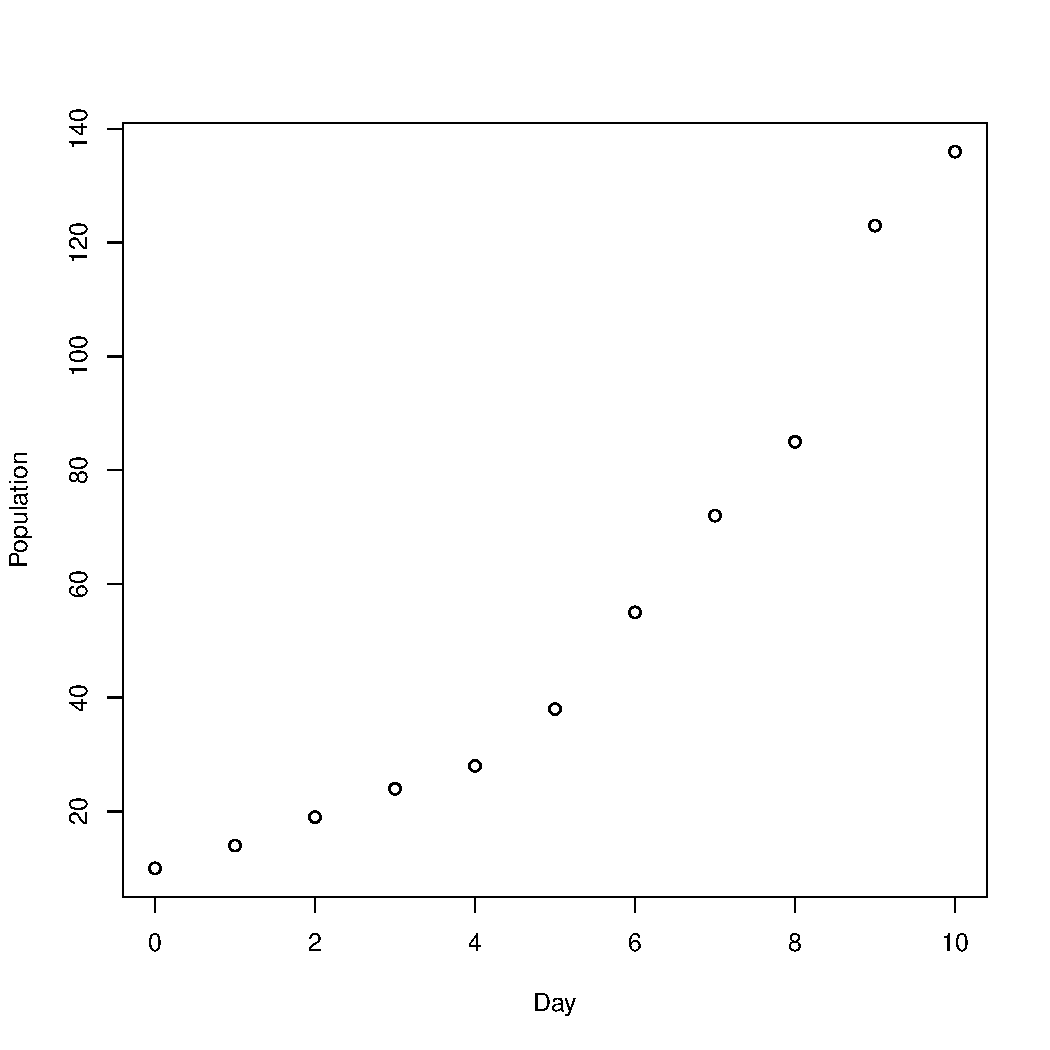
\includegraphics[width=\maxwidth]{figure/unnamed-chunk-2-1} 

\end{knitrout}


b) For more data, use {\bf linear regression}: given\\\ind
$(t_0,P_0), (t_1,P_1),\ldots,(t_{N-1},P_{N-1})$; find $r, \ln(K)$ 
\\\ind to minimize 
$\sum_{n=0}^{N-1}(\ln(P_n)-\ln(K)-rt_n)^2$.\\\vspace{1in}

\newpage\begin{center}{\bf POPULATION GROWTH MODELS CONT.}\end{center}

Example Fruit fly data:\vspace{-3mm}
\begin{verbatim}
Day  0   1   2   3   4   5   6   7   8   9  10 
Pop 10  14  19  24  28  38  55  72  85 123 136
\end{verbatim}
Computer solution: $r\approx .26463$, $K \approx 10.563$ 

%\begin{center}\includegraphics[width=1\textwidth]{fruitfly}\end{center}

\newpage\begin{center}{\bf POPULATION GROWTH MODELS CONT.}\end{center}

Logistic Growth Model: $P' = r(1-P/K)P$. \\
Modeling considers $b$ and $d$ to be dependent on size of $P$;\\
$K$ is {\bf carrying capacity} for population environment.   
\begin{itemize}
\item Qualitative analysis: \\
Equilibrium solutions?\\
Stable or Unstable?\vspace{.5in}

Logistic Equation Solution:\vspace{5.5in}

$$P(t) = K/\big(1+(K/P_0-1)e^{-r(t-t_0)}\big).$$
\end{itemize}
\newpage\begin{center}{\bf POPULATION GROWTH MODELS CONT.}\end{center}

Logistic Model Examples: 

\begin{itemize}
\item $P_0 = 1000$, $P(8)=1200$, eventual $P(t)$ is $20000$.\\\ind
Find $r$, and $t$ when $P(t)$ is 75\% of $K$.\vspace{3.75in}

%\begin{center}\includegraphics[width=.8\textwidth]{logit}\end{center}

\newpage
\item More Fruit Fly Data\vspace{-3mm}
\begin{verbatim}
Day  0   3   7   9  12  15  18  21  24  28  32 
Pop  6  10  21  52  67 104 163 226 265 282 319
\end{verbatim}
Estimate $r$, $K$; and check model.
$$P(t) = K/\big(1+(K/P_0-1)e^{-r(t-t_0)}\big).$$
For $r, K$, use 2 times, e.g. $t = 12, 24$, so\\\ind
\ $67 = K/(1+(K/6-1)e^{-12r})$, and\\\ind
$265 = K/(1+(K/6-1)e^{-24r})$.\\
Eliminate $K$ and solve for $a=e^{-12r}$;

\vspace{1in}

\ind
$K = 67(1-a)/(1-67a/6)$,\\\ind $K = 265(1-a^2)/(1-265a^2/6)$,\\\ind 
$(1-265a^2/6) = 265(1+a)(1-67a/6)/67$;\\\ind
$265/67-1 = 265(61)a/(67\cdot 6);$ $a \approx .0735$, \\$r\approx .218$, 
$K\approx 260?$, not consistent with data.\\

Try other data to find $K,\ r$? \\\ind 
Need to solve nonlinear equation for $r$.\\\ind
Could use nonlinear least-squares fit.
\end{itemize}

US Population Modeling?\\
Can try to fit a logistic model, but predictions not good.\\
Need a model that includes immigration: e.g.
$$P' = r(1-P/K)P + I$$ 
for immigration rate I, or
$$P' = r(t)(1-P/K)P + I(t).$$ 

\end{document}
